% This file was converted to LaTeX by Writer2LaTeX ver. 1.2
% see http://writer2latex.sourceforge.net for more info
\documentclass[11pt]{article}
\usepackage[utf8]{inputenc}
\usepackage[T1]{fontenc}
\usepackage[spanish,english]{babel}
\usepackage{amsmath}
\usepackage{amssymb,amsfonts,textcomp}
\usepackage{array}
\usepackage{supertabular}
\usepackage{hhline}
\usepackage{graphicx}
\makeatletter
\newcommand\arraybslash{\let\\\@arraycr}
\makeatother
\setlength\tabcolsep{1mm}
\renewcommand\arraystretch{1.3}
\newcounter{Figura}
\renewcommand\theFigura{\arabic{Figura}}
\title{}
\begin{document}
  
   \begin{titlepage}

\begin{center}
\vspace*{-1in}

FACULTAD DE INGENIERIA\\
\vspace*{0.15in}
UNIVERSIDAD DE LA REPUBLICA \\
\vspace*{0.6in}
\vspace*{0.2in}
\begin{Large}
\textbf{Análisis} \\
\end{Large}
\vspace*{0.3in}
\end{center}

\begin{minipage}{0.4\textwidth}
\begin{flushleft} \large
\emph{Autor:}\\
Julio Saráchaga\\
\bigskip
\emph{Contraparte del cliente:}\\
Ing. Fernanda Molina
\end{flushleft}
\end{minipage}
\begin{minipage}{0.4\textwidth}
\begin{flushright} \large
\emph{Supervisor:} \\
Dr. Gustavo Betarte\\
\bigskip
\emph{Supervisor alterno:} \\
Ing. Marcelo Rodríguez
\end{flushright}
\end{minipage}\\[3cm]

\end{titlepage}
  
\clearpage\setcounter{page}{1}\section[Introducción]{Introducción}
A continuación se presentan los aspectos más importantes que se tuvieron en cuenta para el desarrollo del proyecto. Se
presentan características deseadas en un sistema de intercambio de información de seguridad entre organizaciones.}

\section{Herramientas}
Luego del estudio del estado del arte, se analizó el problema y se decidieron las herramientas que se utilizarían
considerando la aceptación que pudieran tener por parte de la comunidad. Se consideró el desarrollo actual de dichas
herramientas buscando que tuvieran líneas de trabajo a futuro. A su vez se ha buscado que dichas herramientas cumplan
con los objetivos establecidos al comienzo del proyecto.

\subsection{RTIR}

\bigskip

RTIR es un sistema de manejo de incidentes diseñado para ser utilizado por CERTs y CSIRTs para manejar el creciente
número de incidentes reportados. Si bien existen otras herramientas similares, RTIR presenta la ventaja de ser
opensource y contar con una API que permite extender la herramienta de forma sencilla. RTIR cuenta además con una
comunidad de usuarios grande cuya característica principal es el nivel técnico de estos.

Distintos CERTs y CSIRTs han contribuido en el desarrollo de la herramienta, el resultado ha sido una herramienta que
posee un workflow para el manejo de incidentes de seguridad. Dicho workflow facilita el trabajo de los CERTs y CSIRTs.


\bigskip

El interés de usar RTIR proviene de que el CSIRT-Tilsor \ tiene la herramienta instalada y la utiliza para sus
operaciones. Además hay miembros del equipo que tienen experiencia en su uso. 


Además al ser una herramienta con una profunda inserción en la comunidad, es esperable que sea mas fácil la aceptación
de una extensión basada en TAXII y STIX que la creación de una nueva herramienta a la que los usuarios deberán
adaptarse.


\bigskip


\bigskip

Si bien RTIR fue una premisa dentro de los objetivos del proyecto se evaluaron durante el estudio del arte otras
herramientas que pudieran tomar su lugar. De todas formas del análisis realizado se eligió RTIR por las razones dadas
anteriormente.
 A pesar de utilizarse RTIR, es deseable que la herramienta desarrollada no sea dependiente de RTIR, esto quiere decir
que se pueda utilizar una herramienta con funcionalidades similares en el futuro.


\bigskip


\bigskip

\subsection{STIX y TAXII}

\bigskip

El lenguaje STIX nos provee una representación estructurada de la información de cyber inteligencia que es mas expresiva
que las utilizadas en la actualidad, consta de una mayor flexibilidad y extensibilidad. La representación estructurada
de la información permite el uso de herramientas de automatización sin perder la posibilidad de que la información
representada sea legible.

STIX facilita el intercambio de información entre organizaciones y comunidades. Dicho intercambio se realiza por medio
de TAXII, este protocolo define un conjunto de servicios y mensajes que permiten el intercambio de información entre
organizaciones. El intercambio realizado con TAXII permite la detección, prevención y mitigación de amenazas.


\bigskip

También es importante destacar que STIX facilita la descripción y extensibilidad de evidencia y se integra con otras
iniciativas de MITRE como lo son MAEC y CAPEC. MITRE ha logrado integrar en STIX estas especificaciones en lugar de
reinventar estos componentes. En STIX también se integran otros lenguajes comúnmente utilizados en la comunidad y que
tienen propósitos similares, como los son OpenIOC o IODEF.


\bigskip

Como STIX es un lenguaje XML hereda ciertas propiedades de estos: es un lenguaje extensible, simple y fácil de
procesar.


\bigskip


Además el lenguaje STIX provee expresividad y flexibilidad para expresar intrusiones, técnicas utilizadas por los
adversarios, identificadores de estos entre otras características.


\bigskip

Durante el estudio del estado del arte se evaluaron lenguajes para la representación de información de seguridad de
forma estructurada, así como protocolos para el intercambio de información. Se eligieron STIX y TAXII por ser
iniciativas de MITRE que se integran adecuadamente con otros desarrollos previos de la misma organización. También se
integran adecuadamente con herramientas y lenguajes realizados por otras organizaciones como lo son IODEF de IEEE u
OpenIOC de Mandiant.

Otra de las razones por las cuales se eligieron STIX y TAXII para realizar el proyecto es la consolidación que tiene
MITRE. La organización tiene nexos con otras provenientes tanto del sector publico como privado. Esto causa que los
impulsos realizados por ella tiendan a tener mayor aceptación.

Como se mencionó en el estado del arte, STIX y TAXII han sido desarrollados por los miembros de la comunidad buscando
cubrir las necesidades de los interesados. MITRE tiene el rol de facilitador y coordinador de los esfuerzos realizados
por los participantes del proyecto.


\bigskip

\section[Modelo utilizado]{Módelo utilizado}

\bigskip

La herramienta que se desea desarrollar busca solucionar las problemáticas que se presentan en el intercambio de
información de seguridad entre organizaciones. Dichas problemáticas afectan la reputación, seguridad y la capacidad de
trabajo de la organización. Se pretende desarrollar una herramienta que solucione las problemáticas existentes y que a
su vez pueda ser extendida en un futuro con nuevas funcionalidades.


\bigskip

Para la selección del modelo se estudiaron las características de la organización, se concluyó que el CSIRT-Tilsor es
una organización de investigación que busca tener contacto directo con otros CSIRTs. Además no es una organización
gubernamental ni de coordinación de esfuerzos. Otra de las características que afectan en el modelo del CSIRT es en la
capacidad limitada que tiene la organización de producir y consumir información. Por dichas razones se decidió la
utilización de un modelo ``Peer to Peer'' que permita el establecimiento de acuerdos mutuos para compartir información
entre las organizaciones.

\section{Análisis}

\bigskip

La herramienta que se desea desarrollar busca integrarse con RTIR para realizar un seguimiento de incidentes de
seguridad. Esta herramienta debe permitir el intercambio de indicadores entre dos organizaciones, el cual debe ser
realizado por medio de TAXII con la información representada por medio de STIX. 


\bigskip

Se debería dar la posibilidad de interactuar por medio de RTIR con otros CSIRTs. En dicha interacción se podría realizar
el manejo de incidentes intercambiando información referente a éstos entre los CSIRTs. En dichos intercambios se podría
dar información sobre la identificación , solución, atacantes, etc. Cabe recordar que dichos intercambios hoy en día se
realizan principalmente por medio de foros, email o comunicaciones telefónicas. Se puede ver que la creación de una
herramienta de estas características permitiría el manejo centralizado de la información facilitando el trabajo de los
analistas.


\bigskip

Si bien el intercambio de información no es un problema estrictamente técnico, hay procedimientos y consideraciones
legales y de confianza que podrían afectar el intercambio de información. TAXII y STIX no pretenden solucionar dichos
problemas sino que deben ser tomados en cuenta en los sistemas desarrollados. Por ello es necesario definir políticas
de intercambio de información que especifiquen que puede ser compartido y que no.

Con la finalidad de aplicar dichas políticas se puede sanitizar y anonimizar la información con el fin de remover datos
confidenciales o sensibles antes de que sean compartidos. Para resolver el problema planteado se debe evaluar la
protección que se le quiere dar a la información y de que tanta utilidad es la información luego de ser sanitizada.

Del análisis anterior se desprende la necesidad de contar con un módulo que permita a la aplicación sanitizar la
información. Es deseado que dicha sanitización se alimente de políticas definidas por la organización. La finalidad del
módulo es analizar la información y filtrar datos que pudieran ser sensibles y que pusieran en riesgo los intereses de
la organización.


\bigskip

Otro problema que se presenta en el intercambio de grandes volúmenes de datos es la correlación de información. Si se
tiene información proveniente de diversas fuentes, con datos específicos y referente a distintos tipos de objetos es
deseado \ correlacionar y vincular dicha información con la finalidad de manejar pocos datos los cuales sean más
significativos que los originales.

Un sistema que use correlación busca reducir la carga de trabajo de los analistas y a su vez bajar el periodo de tiempo
entre la detección del problema y su solución.

Con la correlación es posible vincular eventos generados de distintas fuentes para decidir si se tratan de falsos
positivos o hechos reales. A su vez, permite detectar ataques que pudieran pasar desapercibidos en volúmenes muy
grandes de información.


\bigskip

Si bien la información correlacionada es de utilidad para los analistas, puede ser necesario contar con toda la
información recibida para poder hacer un análisis mas profundo de la situación. Por ello es que es necesario que toda
la información que ingrese al sistema sea almacenada de forma independiente a los datos correlacionados. 

Con los datos almacenados, el módulo de correlación aplica las estrategias necesarias para agrupar los datos de forma
adecuada.


\bigskip

Además de recibir información proveniente de socios de la organización es deseable que se pueda ingresar nueva
información al sistema. Se identifican dos posibles métodos de entrada al sistema.

El primero de los métodos identificados es por medio de RTIR, en este un analista ingresa información referente a un
incidente por medio del RTIR. La información es dada de alta en el cliente TAXII y luego es compartida con otros
CSIRTs. El otro método identificado es por medio de sensores dentro de la organización que registren los eventos de la
red. Dichos eventos pueden ser dados de alta en el sistema y compartidos con otros CSIRTs.


\bigskip

De lo anterior podemos resumir los siguientes requerimientos funcionales:


\bigskip

\begin{flushleft}
\tablefirsthead{}
\tablehead{}
\tabletail{}
\tablelasttail{}
\begin{supertabular}{|m{5.83516in}|}
\hline
\centering\arraybslash{\selectlanguage{spanish}\bfseries\color{black} Requerimientos funcionales}\\\hline
\liststyleWWNumii
\begin{itemize}
\item {\selectlanguage{spanish} Agregar políticas de sanitización de la información.}
\item {\selectlanguage{spanish} Aplicación de las políticas de sanitización para la información intercambiada}
\item {\selectlanguage{spanish} Tener la posibilidad de crear información de incidentes de seguridad en el sistema por
medio de RTIR y sensores existentes en la organización.}
\item {\selectlanguage{spanish} Realizar un seguimiento y manejo de incidentes de seguridad.}
\item {\selectlanguage{spanish} La herramienta debe implementar un modelo peer-to-peer de intercambio de información
para la interacción con otros CSIRTs. El intercambio se da por medio de STIX.}
\item {\selectlanguage{spanish} Tener un módulo de correlación de cyber observables.}
\item {\selectlanguage{spanish} Se debe dar la posibilidad de hacer un alta, baja y modificación de servicios TAXII en
otras organizaciones.}
\item {\selectlanguage{spanish} Se debe dar la posibilidad de dar alta, baja y modificación a TAXII Data Feeds de otras
organizaciones.}
\end{itemize}
\\\hline
\end{supertabular}
\end{flushleft}

\bigskip

También se pueden ver los siguientes requerimientos no funcionales:


\bigskip

\begin{flushleft}
\tablefirsthead{}
\tablehead{}
\tabletail{}
\tablelasttail{}
\begin{supertabular}{|m{5.83516in}|}
\hline
\centering\arraybslash{\selectlanguage{spanish}\bfseries\color{black} Requerimientos no funcionales}\\\hline
\liststyleWWNumiii
\begin{itemize}
\item {\selectlanguage{spanish} Extensibilidad: Debe ser posible extender la herramienta con nuevos módulos que
implementen nuevas funcionalidades. Un ejemplo de esto es un modulo de correlación de cyber observables.}
\item {\selectlanguage{spanish} La herramienta debe mantener información en una base de datos independiente a la de
RTIR. Dicha base de datos debe poder representar objetos STIX. Estos objetos podrían ser intercambiados o no.}
\item {\selectlanguage{spanish} Independencia de RTIR}
\end{itemize}
\\\hline
\end{supertabular}
\end{flushleft}

\bigskip


\bigskip


\bigskip


\bigskip

\section{Actores y Casos de Uso}
\subsection{Actores}

\bigskip

\begin{flushleft}
\tablefirsthead{}
\tablehead{}
\tabletail{}
\tablelasttail{}
\begin{supertabular}{m{0.8608598in}m{4.89486in}}
{\selectlanguage{spanish}\color{black} Actor} &
{\selectlanguage{spanish}\color{black} Analista}\\\hline
\multicolumn{1}{m{0.8608598in}|}{{\selectlanguage{spanish}\color{black} Descripción}} &
\multicolumn{1}{m{4.89486in}|}{{\selectlanguage{spanish}\color{black} Este actor tiene la posibilidad de ingresar nueva
información en el sistema. Dicha información puede ser intercambiada con otro sistema. Con la información que se ha
intercambiado el actor puede realizar un análisis de ella y hacer un manejo de los casos creados en el RTIR.}}\\
\end{supertabular}
\end{flushleft}

\bigskip


\bigskip

\begin{flushleft}
\tablefirsthead{}
\tablehead{}
\tabletail{}
\tablelasttail{}
\begin{supertabular}{m{0.8816598in}m{4.8740597in}}
{\selectlanguage{spanish}\color{black} Actor} &
{\selectlanguage{spanish}\color{black} Cliente TAXII}\\\hline
\multicolumn{1}{m{0.8816598in}|}{{\selectlanguage{spanish}\color{black} Descripción}} &
\multicolumn{1}{m{4.8740597in}|}{{\selectlanguage{spanish}\color{black} Este actor es el que interactúa con el sistema
para intercambiar datos por medio del protocolo TAXII. El sistema tiene que dar soporte para dicho protocolo para que
el intercambio sea exitoso.}}\\
\end{supertabular}
\end{flushleft}

\bigskip

\subsection{Casos de uso}
\begin{flushleft}
\tablefirsthead{}
\tablehead{}
\tabletail{}
\tablelasttail{}
\begin{supertabular}{m{1.0573599in}|m{4.82056in}|}
\multicolumn{1}{m{1.0573599in}}{{\selectlanguage{spanish}\color{black} Nombre}} &
\multicolumn{1}{m{4.82056in}}{{\selectlanguage{spanish}\color{black} ABM de políticas}}\\\hline
{\selectlanguage{spanish}\color{black} Actor} &
{\selectlanguage{spanish}\color{black} Analista}\\
{\selectlanguage{spanish}\color{black} Descripción} &
{\selectlanguage{spanish}\color{black} Este caso de uso comienza cuando el analista desea realizar el alta, baja o
modificación con las cuales desee filtrar la información que se desea intercambiar con otras
organizaciones.}\\\hhline{~-}
\end{supertabular}
\end{flushleft}

\bigskip

\begin{flushleft}
\tablefirsthead{}
\tablehead{}
\tabletail{}
\tablelasttail{}
\begin{supertabular}{m{1.0573599in}|m{4.82056in}|}
\multicolumn{1}{m{1.0573599in}}{{\selectlanguage{spanish}\color{black} Nombre}} &
\multicolumn{1}{m{4.82056in}}{{\selectlanguage{spanish}\color{black} ABM de servicios TAXII}}\\\hline
{\selectlanguage{spanish}\color{black} Actor} &
{\selectlanguage{spanish}\color{black} Analista}\\
{\selectlanguage{spanish}\color{black} Descripción} &
{\selectlanguage{spanish}\color{black} Este caso de uso comienza cuando el analista desea realizar el alta, baja o
modificación de servicion TAXII de otras organizaciones en el sistema. Estos serán utilizados para lograr el
intercambio de información.}\\\hhline{~-}
\end{supertabular}
\end{flushleft}

\bigskip


\bigskip

\begin{flushleft}
\tablefirsthead{}
\tablehead{}
\tabletail{}
\tablelasttail{}
\begin{supertabular}{m{0.8816598in}|m{4.8740597in}|}
\multicolumn{1}{m{0.8816598in}}{{\selectlanguage{spanish}\color{black} Nombre}} &
\multicolumn{1}{m{4.8740597in}}{{\selectlanguage{spanish}\color{black} Alta de información RTIR}}\\\hline
{\selectlanguage{spanish}\color{black} Actor} &
{\selectlanguage{spanish}\color{black} Analista}\\
{\selectlanguage{spanish}\color{black} Descripción} &
{\selectlanguage{spanish}\color{black} Este caso de uso comienza cuando el analista desea registrar nueva información en
el sistema. Para ello debe ingresar la información deseada al sistema. Entre la información que puede desear ingresar
se encuentran IPs, hash de archivos, descripciones de amenazas, etc. El manejo podría realizarse por medio de los
incidentes de RTIR.}\\\hhline{~-}
\end{supertabular}
\end{flushleft}

\bigskip

\begin{flushleft}
\tablefirsthead{}
\tablehead{}
\tabletail{}
\tablelasttail{}
\begin{supertabular}{m{0.8816598in}|m{4.8740597in}|}
\multicolumn{1}{m{0.8816598in}}{{\selectlanguage{spanish}\color{black} Nombre}} &
\multicolumn{1}{m{4.8740597in}}{{\selectlanguage{spanish}\color{black} \foreignlanguage{english}{Selección de Taxii Data
Feed}}}\\\hline
{\selectlanguage{spanish}\color{black} Actor} &
{\selectlanguage{spanish}\color{black} Analista}\\
{\selectlanguage{spanish}\color{black} Descripción} &
{\selectlanguage{spanish}\color{black} Con este caso de uso un analista selecciona un data feed en otro sistema al que
quiere subscribirse. Esto se realiza por medio del Feed Managment Service de los sistemas.}\\\hhline{~-}
\end{supertabular}
\end{flushleft}

\bigskip

\begin{flushleft}
\tablefirsthead{}
\tablehead{}
\tabletail{}
\tablelasttail{}
\begin{supertabular}{m{0.8816598in}|m{4.8740597in}|}
\multicolumn{1}{m{0.8816598in}}{{\selectlanguage{spanish}\color{black} Nombre}} &
\multicolumn{1}{m{4.8740597in}}{{\selectlanguage{spanish}\color{black} Recepción de información}}\\\hline
{\selectlanguage{spanish}\color{black} Actor} &
{\selectlanguage{spanish}\color{black} Cliente TAXII}\\
{\selectlanguage{spanish}\color{black} Descripción} &
{\selectlanguage{spanish}\color{black} Este caso de uso se da cuando un cliente TAXII desea enviarle información a
nuestro sistema. El envío de información se realiza porque un analista se subscribió a un data feed en el cliente. La
recepción de información se realiza por medio del Inbox Service de nuestro sistema.}\\\hhline{~-}
\end{supertabular}
\end{flushleft}

\bigskip


\bigskip

\begin{flushleft}
\tablefirsthead{}
\tablehead{}
\tabletail{}
\tablelasttail{}
\begin{supertabular}{m{0.8816598in}|m{4.8740597in}|}
\multicolumn{1}{m{0.8816598in}}{{\selectlanguage{spanish}\color{black} Nombre}} &
\multicolumn{1}{m{4.8740597in}}{{\selectlanguage{spanish}\color{black} Envío de información}}\\\hline
{\selectlanguage{spanish}\color{black} Actor} &
{\selectlanguage{spanish}\color{black} Cliente TAXII}\\
{\selectlanguage{spanish}\color{black} Descripción} &
{\selectlanguage{spanish}\color{black} Este caso de uso se da cuando el sistema desea enviar información a otro cliente
TAXII. El envío de información se realiza porque el cliente se subscribió al TAXII Data Feed del sistema. Esto se
realiza por medio del Inbox Service del cliente. El intercambio es iniciado por el sistema.}\\\hhline{~-}
\end{supertabular}
\end{flushleft}

\bigskip

\begin{flushleft}
\tablefirsthead{}
\tablehead{}
\tabletail{}
\tablelasttail{}
\begin{supertabular}{m{0.8816598in}|m{4.8740597in}|}
\multicolumn{1}{m{0.8816598in}}{{\selectlanguage{spanish}\color{black} Nombre}} &
\multicolumn{1}{m{4.8740597in}}{{\selectlanguage{spanish}\color{black} Poll de información}}\\\hline
{\selectlanguage{spanish}\color{black} Actor} &
{\selectlanguage{spanish}\color{black} Cliente TAXII}\\
{\selectlanguage{spanish}\color{black} Descripción} &
{\selectlanguage{spanish}\color{black} Este caso de uso se da cuando un cliente desea recibir información del sistema en
un intercambio iniciado por él. Este intercambio se realiza por medio del Polling Service del sistema.}\\\hhline{~-}
\end{supertabular}
\end{flushleft}

\bigskip

\begin{flushleft}
\tablefirsthead{}
\tablehead{}
\tabletail{}
\tablelasttail{}
\begin{supertabular}{m{0.8816598in}|m{4.8740597in}|}
\multicolumn{1}{m{0.8816598in}}{{\selectlanguage{spanish}\color{black} Nombre}} &
\multicolumn{1}{m{4.8740597in}}{{\selectlanguage{spanish}\color{black} Poll de información a un cliente TAXII}}\\\hline
{\selectlanguage{spanish}\color{black} Actor} &
{\selectlanguage{spanish}\color{black} Cliente TAXII}\\
{\selectlanguage{spanish}\color{black} Descripción} &
{\selectlanguage{spanish}\color{black} Este caso de uso se da cuando el sistema desea recibir información de un cliente
TAXII en un intercambio iniciado por él. Este intercambio se realiza por medio del Polling Service del
sistema.}\\\hhline{~-}
\end{supertabular}
\end{flushleft}

\bigskip

{\selectlanguage{spanish}
También se deben considerar los casos de uso provistos por RTIR para el seguimiento y manejo de los incidentes los
cuales no son especificados. Dichos casos de uso permiten el manejo de tickets y queues. Alta y baja de usuarios en
RTIR. }

{\selectlanguage{spanish}
Con RTIR se especifica un workflow para el trabajo con los tickets en organizaciones de seguridad. Dicho workflow
comienza cuando se reporta un incidente, dicho reporte de incidente se asocia a un incidente o se crea uno nuevo. Los
incidentes tratan de registrar toda la información necesaria para resolver el problema. De los incidentes se pueden
iniciar investigaciones para trabajar con otras organizaciones. También se pueden crear blocks para mantener un
registro de los que se ha realizado para mitigar el incidente.}


\bigskip

\subsection{Comportamiento de casos de uso}
\subsubsection{Diagrama de casos de uso}
{\selectlanguage{spanish}
En el siguiente diagrama se ve en resumen los actores y casos de uso del sistema}

 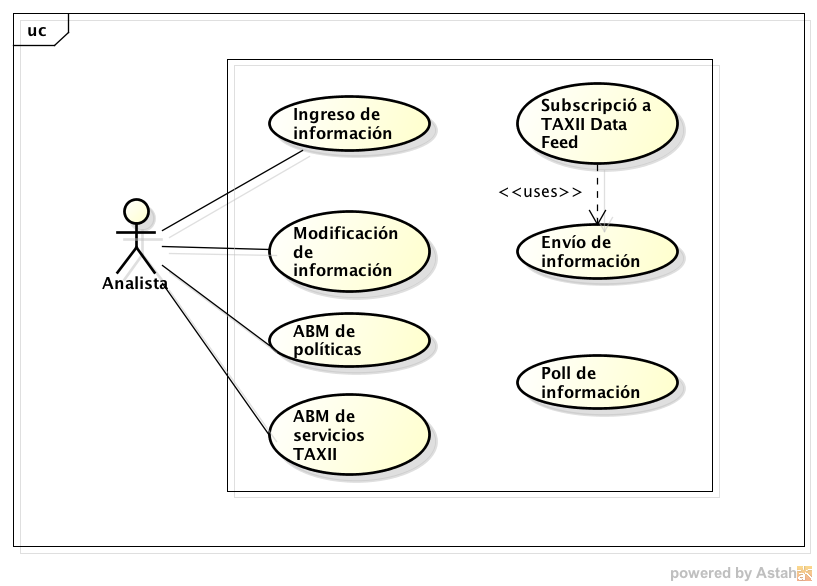
\includegraphics[width=5.7638in,height=4.1339in]{Analisis21-img006.png} 

{\centering\selectlanguage{english}\bfseries
\foreignlanguage{spanish}{Figura }\stepcounter{Figura}{\theFigura}\foreignlanguage{spanish}{ - Diagrama de caso de uso}
\par}

\subsubsection{Diagramas de Secuencia del Sistema}

\bigskip

{\selectlanguage{spanish}
A continuación se presentan los diagramas de secuencia del sistema para los casos de uso. En los casos de uso que son
similares no se presentan los diagramas.}

 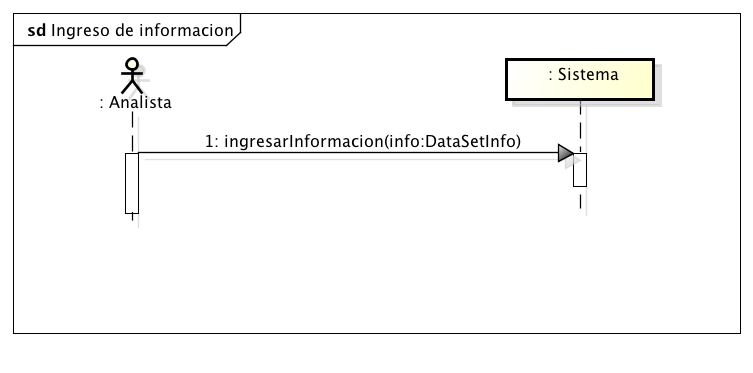
\includegraphics[width=5.7638in,height=2.8547in]{Analisis21-img007.png} 

{\centering\selectlanguage{english}\bfseries
\foreignlanguage{spanish}{Figura }\stepcounter{Figura}{\theFigura}\foreignlanguage{spanish}{ - caso de uso de ingreso de
información}
\par}

 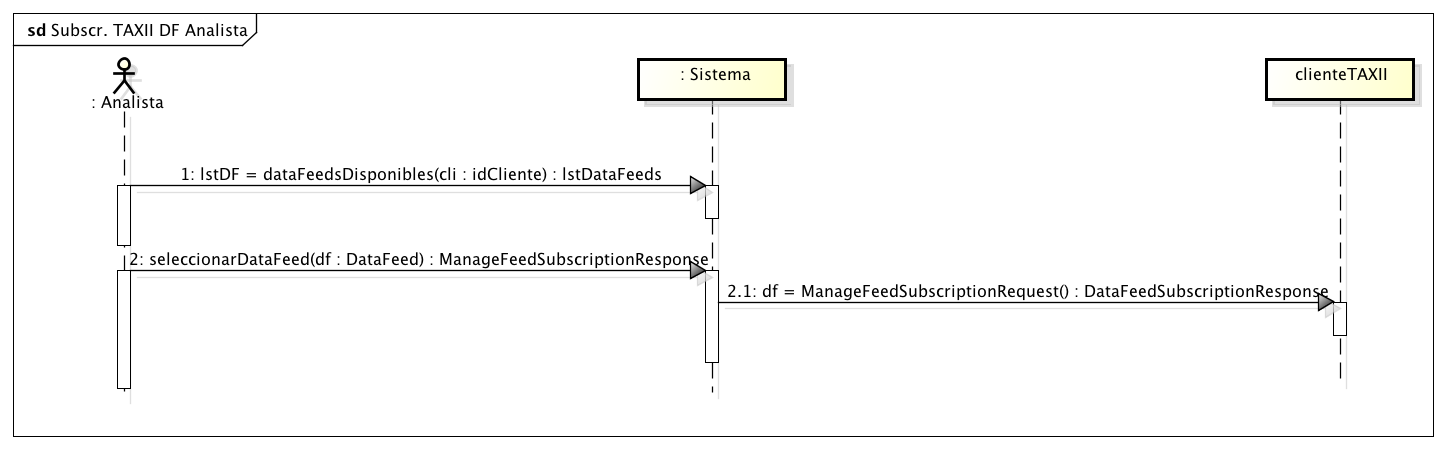
\includegraphics[width=5.7638in,height=1.8965in]{Analisis21-img008.png} 

{\centering\selectlanguage{english}\bfseries
\foreignlanguage{spanish}{Figura }\stepcounter{Figura}{\theFigura}\foreignlanguage{spanish}{ - Caso de uso subscribirse
a un Data Feed} 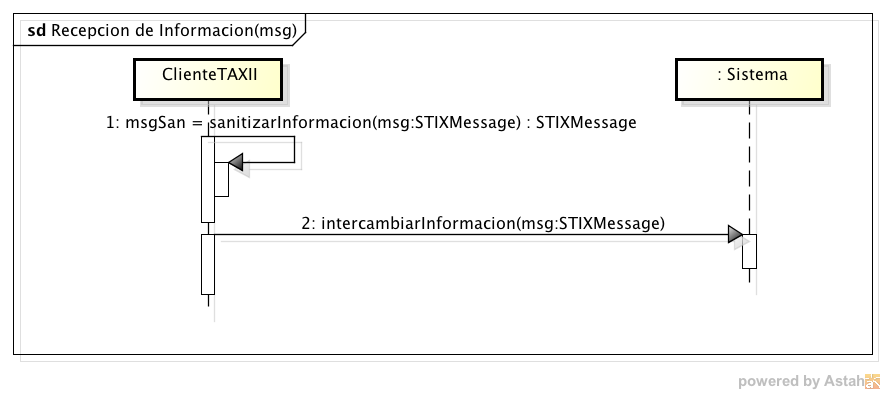
\includegraphics[width=5.7638in,height=2.5661in]{Analisis21-img009.png} 
\par}

{\centering\selectlanguage{english}\bfseries
\foreignlanguage{spanish}{Figura }\stepcounter{Figura}{\theFigura}\foreignlanguage{spanish}{ - Caso de uso de recepción
de información} 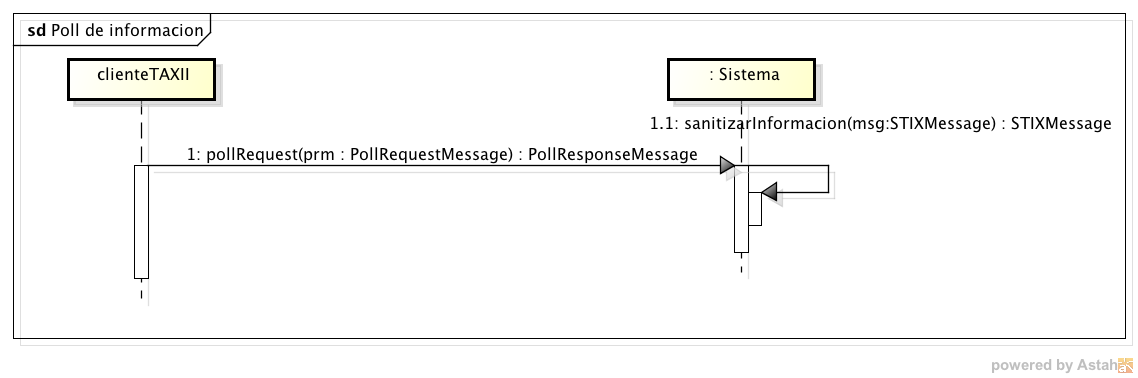
\includegraphics[width=5.7638in,height=1.9146in]{Analisis21-img010.png} 
\par}

{\centering\selectlanguage{english}\bfseries
\foreignlanguage{spanish}{Figura }\stepcounter{Figura}{\theFigura}\foreignlanguage{spanish}{ - Caso de uso poll de
información}
\par}

\subsubsection{Contratos}

\bigskip

\begin{flushleft}
\tablefirsthead{}
\tablehead{}
\tabletail{}
\tablelasttail{}
\begin{supertabular}{|m{1.0115598in}|m{4.7441597in}|}
\hline
{\selectlanguage{spanish}\bfseries Nombre} &
{\selectlanguage{spanish}\bfseries ingresarInformacion}\\\hline
{\selectlanguage{spanish}\bfseries Operación} &
{\selectlanguage{spanish} ingresarInformacion(info:DataSetInfo)}\\\hline
{\selectlanguage{spanish}\bfseries Entrada} &
{\selectlanguage{spanish} Info representa los datos de la información que se desea ingresar al sistema.}\\\hline
{\selectlanguage{spanish}\bfseries Salida} &
{\selectlanguage{spanish} No aplica}\\\hline
{\selectlanguage{spanish}\bfseries Descripción} &
{\selectlanguage{spanish} Ingresa al sistema la información que el analista desee agregar.}\\\hline
\end{supertabular}
\end{flushleft}

\bigskip

\begin{flushleft}
\tablefirsthead{}
\tablehead{}
\tabletail{}
\tablelasttail{}
\begin{supertabular}{|m{1.0115598in}|m{4.7441597in}|}
\hline
{\selectlanguage{spanish}\bfseries Nombre} &
{\selectlanguage{spanish}\bfseries dataFeedsDisponibles}\\\hline
{\selectlanguage{spanish}\bfseries Operación} &
{\selectlanguage{spanish} lstDF := dataFeedsDisponibles(cli : idCliente) : lstDataFeed}\\\hline
{\selectlanguage{spanish}\bfseries Entrada} &
{\selectlanguage{spanish} Se pasa como parámetro el id del cliente en el sistema.}\\\hline
{\selectlanguage{spanish}\bfseries Salida} &
{\selectlanguage{spanish} Se retorna una lista de los DataFeeds en dicho sistema.}\\\hline
{\selectlanguage{spanish}\bfseries Descripción} &
{\selectlanguage{spanish} La operación retorna una lista con los DataFeeds existentes en el cliente pasado como
parámetro.}\\\hline
\end{supertabular}
\end{flushleft}

\bigskip

\begin{flushleft}
\tablefirsthead{}
\tablehead{}
\tabletail{}
\tablelasttail{}
\begin{supertabular}{|m{1.0115598in}|m{4.7441597in}|}
\hline
{\selectlanguage{spanish}\bfseries Nombre} &
{\selectlanguage{spanish}\bfseries seleccionarDataFeed}\\\hline
{\selectlanguage{spanish}\bfseries Operación} &
{\selectlanguage{spanish} seleccionarDataFeed(df : DataFeed) : msg}\\\hline
{\selectlanguage{spanish}\bfseries Entrada} &
{\selectlanguage{spanish} El parámetro df representa un DataFeed en un cliente TAXII.}\\\hline
{\selectlanguage{spanish}\bfseries Salida} &
{\selectlanguage{spanish} Se retorna un mensaje de éxito o error.}\\\hline
{\selectlanguage{spanish}\bfseries Descripción} &
{\selectlanguage{spanish} La operación trata de suscribir el sistema a un nuevo TAXII Data Feed en un cliente
TAXII.}\\\hline
\end{supertabular}
\end{flushleft}

\bigskip

\begin{flushleft}
\tablefirsthead{}
\tablehead{}
\tabletail{}
\tablelasttail{}
\begin{supertabular}{|m{1.0115598in}|m{4.7441597in}|}
\hline
{\selectlanguage{spanish}\bfseries Nombre} &
{\selectlanguage{spanish}\bfseries ManageFeedSubscriptionRequest}\\\hline
{\selectlanguage{spanish}\bfseries Operación} &
{\selectlanguage{spanish} Df := ManageFeedSubscriptionRequest() : DataFeedSubscriptionResponse}\\\hline
{\selectlanguage{spanish}\bfseries Entrada} &
~
\\\hline
{\selectlanguage{spanish}\bfseries Salida} &
{\selectlanguage{spanish} Se retorna un mensaje Feed Subscription Response Message con el resultado de la
operación.}\\\hline
{\selectlanguage{spanish}\bfseries Descripción} &
{\selectlanguage{spanish} La operación se lleva a acabo entre un cliente TAXII y el otro. El cliente trata de
subscribirse en el otro para así poder intercambiar información.}\\\hline
\end{supertabular}
\end{flushleft}

\bigskip


\bigskip
\newpage
\begin{flushleft}
\tablefirsthead{}
\tablehead{}
\tabletail{}
\tablelasttail{}
\begin{supertabular}{|m{1.0115598in}|m{4.7441597in}|}
\hline
{\selectlanguage{spanish}\bfseries Nombre} &
{\selectlanguage{spanish}\bfseries intercambiarInformacion}\\\hline
{\selectlanguage{spanish}\bfseries Operación} &
{\selectlanguage{spanish} intercambiarInformacion(msg:STIXMessage)}\\\hline
{\selectlanguage{spanish}\bfseries Entrada} &
{\selectlanguage{spanish} Se recibe como parámetro un mensaje STIX.}\\\hline
{\selectlanguage{spanish}\bfseries Salida} &
~
\\\hline
{\selectlanguage{spanish}\bfseries Descripción} &
{\selectlanguage{spanish} La operación envía al Inbox Service de otro cliente un mensaje STIX. Este incluye la
información de seguridad a intercambiar.}\\\hline
\end{supertabular}
\end{flushleft}

\bigskip

\begin{flushleft}
\tablefirsthead{}
\tablehead{}
\tabletail{}
\tablelasttail{}
\begin{supertabular}{|m{1.0115598in}|m{4.7441597in}|}
\hline
{\selectlanguage{spanish}\bfseries Nombre} &
{\selectlanguage{spanish}\bfseries pollRequest}\\\hline
{\selectlanguage{spanish}\bfseries Operación} &
{\selectlanguage{spanish} pollRequest(prm:PollRequestMessage) : pollResponseMessage}\\\hline
{\selectlanguage{spanish}\bfseries Entrada} &
{\selectlanguage{spanish} Prm representa la información que se desea recibir del servidor.}\\\hline
{\selectlanguage{spanish}\bfseries Salida} &
{\selectlanguage{spanish} Se retorna la información que se pidió por medio de prm.}\\\hline
{\selectlanguage{spanish}\bfseries Descripción} &
{\selectlanguage{spanish} La operación retorna la información deseada, \ el prm es el que identifica la información en
el servidor.}\\\hline
\end{supertabular}
\end{flushleft}

\bigskip


\bigskip
\end{document}
